\chapter{Requirements \& Design Drivers}





The requirements for the system were derived through a
three-level flow-down from stakeholder needs to mission requirements
to system requirements.

The key design drivers are summarized in Table~\ref{tab:key_reqs}.
Several requirements contained TBD values and have been updated.\\


\begingroup
\small
\setlength{\LTpre}{0pt}
\setlength{\LTpost}{0pt}

\begin{xltabular}{\textwidth}{@{}p{0.28\textwidth} p{0.14\textwidth} X@{}}
\caption{BELLONA key system requirements}
\label{tab:key_reqs}\\

\toprule
\textbf{ID} & \textbf{Change} & \textbf{Requirement} \\
\midrule
\endfirsthead

\caption[]{BELLONA Key System Requirements (continued)}\\
\toprule
\textbf{ID} & \textbf{Change} & \textbf{Requirement} \\
\midrule
\endhead

\bottomrule
\endlastfoot

REQ-STK-01-MSN-01-SYS-01 &
TBD Updated &
The system shall take less than 25 minutes from the balloon
entering the covered airspace to the balloon being removed
from the endangered airspace. \\

\addlinespace
REQ-STK-03-MSN-04-SYS-07 &
Existing &
The system shall be capable of autonomously intercepting
the detected balloon. \\

\addlinespace
REQ-STK-03-MSN-04-SYS-08 &
Existing &
The system shall be capable of intercepting the detected
balloon at an altitude of up to 6000 m. \\

\addlinespace
REQ-STK-05-MSN-06-SYS-11 &
Existing &
The system shall be capable of controlling an intercepted
balloon with a payload mass up to 50 kg. \\

\addlinespace
REQ-STK-05-MSN-06-SYS-13 &
Existing &
The system shall be capable of autonomously delivering
The payload to the selected safe landing zone within 10 m. \\

\addlinespace
REQ-STK-10-MSN-12-SYS-22 &
Updated &
The system shall cost less than EUR~25,000, adjusted to
1 January 2026, for all flying components. \\

\addlinespace
REQ-STK-11-MSN-13-SYS-23 &
Existing &
The system cost per sortie shall be less than EUR~500, adjusted to
1 January 2026. \\

\addlinespace
REQ-STK-12-MSN-15-SYS-27 &
Existing &
The system shall operate in compliance with all applicable
aviation regulations in the operating airspace. \\

\addlinespace
REQ-STK-03-MSN-04-SYS-44 &
\textbf{Added} &
The system shall be capable of intercepting the detected
balloon at a horizontal ground range of up to 6000 m from the
launch or deployment location. \\

\addlinespace
REQ-STK-01-MSN-01-SYS-45 &
\textbf{Added} &
The system shall be capable of safely interacting with balloon-payload configurations with a payload-to-balloon tether length between 0.1 m and 35 m. \\

\addlinespace
REQ-STK-07-MSN-09-SYS-46 &
\textbf{Added} &
The system shall be capable of performing the interception and
recovery mission in sustained winds up to 13 m/s and gusts up to
to 21 m/s. \\
\end{xltabular}
\endgroup




\noindent The main feasibility challenge is the combination of
a low-cost unmanned aerial platform with controlled interaction
and recovery of a large, uncertain, and possibly heavy
balloon-payload system.


\subsection*{Radar Detection Range}
Existing airport surveillance radar, complemented where available by
mobile bird- or drone-detection radar- is treated as the first cueing
layer. The ASR-11 airport surveillance radar is used as a
representative reference system because its parameters are well
documented.

Balloon detectability depends mainly on radar cross-section (RCS), $\sigma$.
Representative RCS values for a $1.5\,\text{m}$ air balloon are given
in \autoref{tab:rcs_values}; these values support the cueing discussion
    but do not redefine the 2--6 m target envelope, defined in
\autoref{tab:key_reqs}. The ASR-11 parameters used for the first-order
range estimate are summarised in \autoref{tab:asr11_parameters}. The
wavelength $\lambda$ is obtained from the radar frequency, and
$S_{min}$ is assumed to correspond to $10\,\text{dB}$ above the noise
floor.

\begin{table}[ht]
    \centering
    \begin{minipage}{0.45\textwidth}
        \centering
        \caption{Average RCS values of air balloon \cite{HUANG2024DetectionRadar.}.}
        \label{tab:rcs_values}
        \begin{tabular}{lc}
            \toprule
            Band & Average RCS ($m^2$) \\
            \midrule
            L  & $4.4618 \times 10^{-5}$ \\
            S  & $3.0878 \times 10^{-4}$ \\
            C  & $6.1819 \times 10^{-4}$ \\
            X  & $9.8522 \times 10^{-4}$ \\
            Ku & $1.6000 \times 10^{-3}$ \\
            \bottomrule
        \end{tabular}
    \end{minipage}
    \hfill
    \begin{minipage}{0.5\textwidth}
        \centering
        \caption{ASR-11 system parameters \cite{ForecastInternational2014ASR-11DASROrientation}.}
        \label{tab:asr11_parameters}
        \begin{tabular}{lcc}
            \toprule
            \textbf{Parameter} & \textbf{Sym.} & \textbf{Value} \\
            \midrule
            Peak Power & $P_t$ & $25 \times 10^3$ W \\
            Antenna Gain & $G$ & 34 dB \\
            Wavelength (S band) & $\lambda$ & $\approx 0.1034$ m \\
            Min. Signal Power & $S_{min}$ & $1 \times 10^{-13}$ W \\
            Hor. Beamwidth &  $ \theta$ & $1.4$ rad \\
            Ver. Beamwidth & $\varphi$ &  $5$ rad\\
            Pulsewidth (short) & $T_{short}$& $1 \mu\text{s}$\\ 
            
            \bottomrule
        \end{tabular}
    \end{minipage}
\end{table}



The maximum detection range is estimated by requiring the received reflected power to exceed the minimum detectable threshold. Using the monostatic radar range equation,

\begin{equation}
    R_{max}=\sqrt[4]{\frac{P_tG^2\lambda^2\sigma}{(4\pi)^3S_{min}}},
\end{equation}

The resulting value of almost \textbf{7200} meters for an undisturbed
clear-weather case with limited clutter or interference. This is an
idealized first-order estimate for early sizing.

The same method can be applied to mobile bird- and drone-detection
radars in areas without permanent airport radar coverage. For example,
The Robin Iris X-band radar is listed for shorter-range small-target
detection \cite{BirdRadar}; a preliminary calculation gives a range
consistent with the manufacturer-stated value of approximately
$3700\,\text{m}$ for small drones. This Value for the radar range was used to determine the mission horizontal range. The detected signal will be classified into a radar chunk, which is characterized by the resolution range, calculated using the time of short Pulsewidth and the speed of the electromagnetic wave, and is equal to $150$ meters. It is further limited by the horizontal and vertical beamwidths. The mission region and the radar chunks are presented in the \autoref{fig:radar detection} 
\begin{figure}[h]
    \centering
    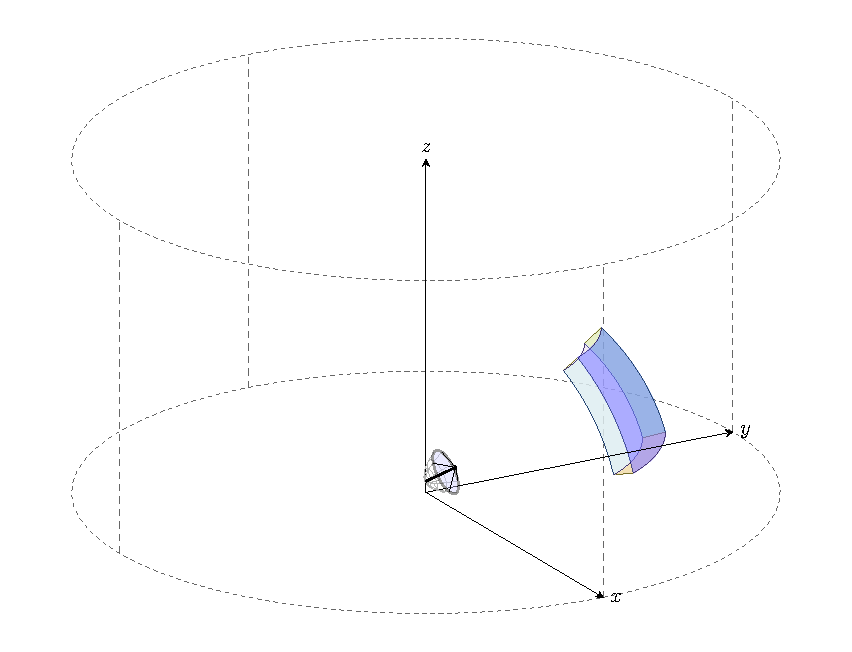
\includegraphics[width=0.5\linewidth]{figures/Radar_det.pdf}
    \caption{Mission Region and example radar chunk}
    \label{fig:radar detection}
\end{figure}
